\documentclass[notitlepage]{report}
\usepackage{hyperref}
\usepackage{tikz}
\usetikzlibrary{calc}

\usepackage{chapterbib}

\setlength{\textwidth}{6.5in}
\setlength{\oddsidemargin}{0in}
\setlength{\evensidemargin}{0in}
\setlength{\topmargin}{-.5in}
\setlength{\headheight}{0in}
\setlength{\textheight}{9in}

\usepackage{amsmath,amssymb,amsfonts}
\usepackage{graphicx}
\usepackage{xcolor}
%\usepackage{wrapfig}

%\setcitestyle{square, numbers}

%% MACROS FOR CHANGING ISSUES IN CODE
\newcommand{\mypaper}{\href{}{Boston (2022)}}
\def\myemail{rboston628@gmail.com}
\def\updatedate{(07/15/2021) }
\def\version{1.0}

%make typewritten zeros correct
\usepackage[T1]{fontenc}
\usepackage[scaled]{inconsolata}%use either inconsolata or beramono

%basic commands
\newcommand{\into}{\rightarrow}
\newcommand{\abs}[1]{\left\vert #1 \right\vert}

%derivaties
\newcommand{\del}[2]{\frac{\partial#1}{\partial #2}}
\newcommand{\dif}[2]{\frac{d#1}{d#2}}

%vector stuff
\newcommand{\m}[1]{\mathbf{#1}}
\newcommand{\mxi}{\boldsymbol{\xi}}
%\newcommand{\bs}[1]{\boldsymbol{#1}}
\newcommand{\dotprod}{\boldsymbol{\cdot}} % the typical scalar product

\newcommand{\Mstar}{M_\star}
\newcommand{\Rstar}{R_\star}
\newcommand{\Lstar}{L_\star}
\newcommand{\Msolar}{M_\odot}
\newcommand{\Rsolar}{R_\odot}
\newcommand{\Lsolar}{L_\odot}
\newcommand{\ad}{\text{ad}}
\newcommand{\rad}{\text{rad}}


\setcounter{section}{0}
\setcounter{subsection}{0}




%1.a.b
\renewcommand{\labelenumi}{\arabic{enumi}.}
\renewcommand{\labelenumii}{(\alph{enumii})}
\renewcommand{\labelenumiii}{(\alph{enumiii})}

\newcommand{\tclass}[1]{\text{\tt#1}}
\newcommand{\tcode}[1]{\text{\tt#1}}
\newcommand{\tfile}[1]{\text{\tt#1}}

%%%%%%%%%%%%%%%%%%%%%%%%%%%%%%%%%%%%%%%%
%%%%%%%%%%%%%%%%%%%%%%%%%%%%%%%%%%%%%%%%

\begin{document}


\title{GRPulse Documentation v\version}
\date{\today}
%\received{}

\author{S.~Reece Boston\footnote{\href{mailto:\myemail}{\myemail}}}
\maketitle

\section*{Diagrammatic Table of Contents}
Click on a box in the below code diagram to jump to the relevant chapter.  Green boxes are not yet included.
\begin{center}
\begin{tikzpicture}
	\def\height{10};
	\def\width{7};
	\coordinate (stars) at (       0,\height);
	\coordinate (drivs) at (  \width,\height);
	\coordinate (modes) at (2*\width,\height);
	\coordinate (over) at (1,0);
	\coordinate (down) at (0,-1);
%% STELLAR MODELS
	\node[anchor=north] (SS) at ($(stars)+(0.2,0)$) {};
	\node[anchor=west,thick, color=red,   rectangle,draw] (STAR) at (stars) {\hyperlink{class:Star}{Star}};
	\node[anchor=west,thick, color=black, rectangle,draw] (Polytrope) at ($(stars)+(over)+1*(down)$) {\hyperlink{class:Polytrope}{Polytrope}};
	\node[anchor=west,thick, color=black, rectangle,draw] (MESA)      at ($(stars)+(over)+2*(down)$) {\hyperlink{class:MESA}{MESA}};
	\node[anchor=west,thick, color=black, rectangle,draw] (CHWD)      at ($(stars)+(over)+3*(down)$) {\hyperlink{class:CHWD}{ChandrasekharWD}};
	\node[anchor=west,thick, color=green, rectangle,draw] (ZAMS)      at ($(stars)+(over)+4*(down)$) {ZAMS};
	\node[anchor=west,thick, color=green, rectangle,draw] (SWD)       at ($(stars)+(over)+5*(down)$) {SimpleWD};
	%%PN
	\node[anchor=north] (PNS) at ($(stars)+(over)+6*(down)+(0.2,0)$) {};
	\node[anchor=west,thick, color=red,   rectangle,draw] (PNStar)      at ($(stars)+1*(over)+6*(down)$) {\hyperlink{class:PNStar}{PNStar}};
	\node[anchor=west,thick, color=black, rectangle,draw] (PNPolytrope) at ($(stars)+2*(over)+7*(down)$) {\hyperlink{class:PNPolytrope}{PNPolytrope}};
	\node[anchor=west,thick, color=black, rectangle,draw] (PNCHWD)      at ($(stars)+2*(over)+8*(down)$) {\hyperlink{class:PNChandrasekharWD}{PNChandrasekharWD}};
	%%GR
	\node[anchor=north] (GRS) at ($(stars)+(over)+9*(down)+(0.2,0)$) {};
	\node[anchor=west,thick, color=red,   rectangle,draw] (GRStar)      at ($(stars)+1*(over)+9*(down)$) {\hyperlink{class:GRStar}{GRStar}};
	\node[anchor=west,thick, color=black, rectangle,draw] (GRPolytrope) at ($(stars)+2*(over)+10*(down)$) {\hyperlink{class:GRPolytrope}{GRPolytrope}};
	\node[anchor=west,thick, color=green, rectangle,draw] (GRCHWD)      at ($(stars)+2*(over)+11*(down)$) {GRChandrasekharWD};
	%draw the legs
	\draw[->] (SS) |- (Polytrope.west);
	\draw[->] (SS) |- (MESA.west);
	\draw[->] (SS) |- (CHWD.west);
	\draw[->] (SS) |- (ZAMS.west);
	\draw[->] (SS) |- (SWD.west);
	%
	\draw[->] (SS)  |- (PNStar.west);
	\draw[->] (PNS) |- (PNPolytrope.west);
	\draw[->] (PNS) |- (PNCHWD.west);
	%
	\draw[->] (SS)  |- (GRStar.west);
	\draw[->] (GRS) |- (GRPolytrope.west);
	\draw[->] (GRS) |- (GRCHWD.west);
	
%% MODE DRIVERS
	\node[anchor=north] (MD) at ($(drivs)+(0.2,0)$) {};
	\node[anchor=west,thick,color=red, rectangle, draw] (DRV) at (drivs) {\hyperlink{class:ModeDriver}{ModeDriver}};
	\node[anchor=west,thick,color=black,rectangle,draw] (Cowling)     at ($(drivs)+(over)+1*(down)$) {\hyperlink{class:CowlingModeDriver}{CowlingModeDriver}};
	\node[anchor=west,thick,color=black,rectangle,draw] (Full)        at ($(drivs)+(over)+2*(down)$) {\hyperlink{class:NonradialModeDriver}{NonradialModeDriver}};
	%
	\node[anchor=west,thick,color=black,rectangle,draw] (PNNonradialMode)  at ($(drivs)+(over)+7*(down)$) {\hyperlink{class:PNNonradialModeDriver}{PNNonradialModeDriver}};
	%
	\node[anchor=west,thick,color=black,rectangle,draw] (GRCowlingMode)  at ($(drivs)+(over)+10*(down)$) {\hyperlink{class:GRCowlingModeDriver}{GRCowlingModeDriver}};
	\node[anchor=west,thick,color=green,rectangle,draw] (GRNonradialMode)  at ($(drivs)+(over)+11*(down)$) {GRNonradialModeDriver};
	\draw[->] (MD) |- (Cowling.west);
	\draw[->] (MD) |- (Full.west);
	\draw[->] (MD) |- (PNNonradialMode.west);
	\draw[->] (MD) |- (GRCowlingMode.west);
	\draw[->] (MD) |- (GRNonradialMode.west);
	
%% MODE, BY ITSELF
	\node[anchor=west,thick,color=black,rectangle,draw] (MODE) at (modes) {\hyperlink{class:Mode}{Mode\texttt{<N>}}};
	%list mode variable numbers
	\node[anchor=west, rectangle,draw] at ($(modes)+1*(down)$) {N=2} edge[<-,color=blue,dashed] (Cowling.east);
	\node[anchor=west, rectangle,draw] at ($(modes)+2*(down)$) {N=4} edge[<-,color=blue,dashed] (Full.east);
	\node[anchor=west, rectangle,draw] at ($(modes)+7*(down)$) {N=8} edge[<-,color=blue,dashed] (PNNonradialMode.east);
	\node[anchor=west, rectangle,draw] at ($(modes)+10*(down)$) {N=2} edge[<-,color=blue,dashed] (GRCowlingMode.east);
	\node[anchor=west, rectangle,draw] at ($(modes)+11*(down)$) {N=4$\mathbb{C}$/8$\mathbb{R}$} edge[<-,color=blue,dashed] (GRNonradialMode.east);
	
	%%connect friends
	\draw[color=blue,->] (STAR.east) to node[anchor=south] {$\rho,P,m,\Phi$, etc.} node[anchor=north] {boundary expansions} (DRV.west);
	\draw[color=blue,->] (DRV.east) to node[anchor=south] {$A^\ast, V_g, U, c_1$, etc.} node[anchor=north] {boundary conditions} (MODE.west);
	\draw[color=blue,->] (PNStar.east) to node[anchor=south] {$d\Psi/dr$, etc.} ($(drivs)+6*(down)$);
	\draw[color=blue,->] (GRStar.east) to node[anchor=south] {$g_{ab}, \nu, \lambda$, etc.} ($(drivs)+9*(down)$);
\end{tikzpicture}
\end{center}


\tableofcontents


\chapter{Introduction}
This document contains development notes and user notes for the \tcode{GRPulse} program developed as part of my thesis work.  This document explains the equations and algorithms used, why certain choices are made, and how to use and further develop the program.

\section{How to Cite This Program}
If you use this program in scientific research, please cite it by the paper introducing it: \mypaper

In bibtex
\begin{verbatim}
@PHDTHESIS{Boston2022,
	title = {Newtonian and Relativistic White Dwarf Asteroseismology},
	author = {Boston, S.~Reece},
	school = {University of North Carolina},
	year = {2022}
}
\end{verbatim}



\section{Version \version}
This documentation was created for release with version \version, which was released with the above paper.  Later updates will include functionality for realistic simple WD models, and for asteroseismology in full general relativity.

\section{Structure of Program}

The program follows OOP design.  Most control of the program is contained within methods attached to classes.  The classes act to encapsulate data and methods.

One of the benefits of OOP design is polymorphism; the ability to use different classes interchangeably.  This is facilitated by the use of abstract classes. There are three main abstract classes in the code:
\begin{itemize}
\item \tclass{Star}: Represents an equilibrium model of a star used as background in the wave equations.
Described in \ref{class:Star}.
\item \tclass{Mode<N>}: Represents a single $klm$-mode, described by an \tcode{N}-dimensional eigenfunction (e.g. for a Cowling mode \tcode{N}=2).
Described in \ref{class:Mode}.
\item \tclass{ModeDriver}: Represents a particular form of a stellar wave equation (e.g. Cowling modes, Dziembowski equations, or non-adiabatic waves). 
Described in \ref{class:ModeDriver}.
\end{itemize}
Classes \tclass{Star} and \tclass{ModeDriver} are abstract, meaning they only provide a template that other classes have to follow.
It is up to the children of \tclass{Star} and \tclass{ModeDriver} to actually implement those methods.

The structure of the code, the polymorphism pattern, and the relationship between the classes, is illustrated in Figure \ref{fig:struct}.

In this document, we separate two facets of the classes, as they relate to the OOP structure:
\begin{description}
	\item[Interface] External-facing elements (data or functions) that specify how outside code can interact with the object.
	\item[Implementation] The internal logic that calculates all relevant values inside of the object, and cannot be seen by external code.
\end{description}
As an example, all \tclass{Star}s have an method \tcode{rho()} in their interface, which must return the density $\rho$; however, the implementation can vary on how $\rho$ is found, whether by storing $\rho$ in an array, or calculating it from other quantities.  
 
This is illustrated in Figure \ref{fig:interface}.

\begin{figure}[h]
\hfill
\begin{tikzpicture}
  \draw[thick] (0,0) rectangle (4,5);
  \node[thick, anchor=south west] at (0,0) {\tclass{Star}};
  \draw[thick] (4,4) rectangle (6, 4.5);
  \draw[thick] (4,2) rectangle (5, 2.5);
  \node[thick, anchor=south east] at (6,4) {\tcode{rho()}};
  \node[thick, anchor=south east] at (5,2) {\tcode{P()}};

  \draw[thick,color=red] (0.5,0.5) rectangle (3.5,4.5);
  \node[thick, color=red, anchor=south west] at (0.5,0.5) {\tclass{Polytrope}};
  \draw[color=red] (2, 3.2) ellipse [x radius=1.25,y radius=0.5];
  \draw[color=red] (2, 2) ellipse [x radius=1.25, y radius=0.5];
  \node[color=red] at (2,3.2) {$\rho = \rho_c\theta^n$};
  \node[color=red] at (2,2) {$P = P_c \theta^{n+1}$};
  \draw[thick, color=red, ->] (3,3.2) -| (3.75, 4.25) -- (4, 4.25);
  \draw[thick, color=red, ->] (3,2) -| (3.75, 2.25) -- (4, 2.25);
\end{tikzpicture}
\hfill
\begin{tikzpicture}
  \draw[thick] (0,0) rectangle (4,5);
  \node[thick, anchor=south west] at (0,0) {\tclass{Star}};
  \draw[thick] (4,4) rectangle (6, 4.5);
  \draw[thick] (4,2) rectangle (5, 2.5);
  \node[thick, anchor=south east] at (6,4) {\tcode{rho()}};
  \node[thick, anchor=south east] at (5,2) {\tcode{P()}};

  \draw[thick,color=green] (0.5,0.5) rectangle (3.5,4.5);
  \node[thick, color=green, anchor=south west] at (1,1) {\tclass{MESA}};
  \draw[color=green] (2, 3.2) ellipse [x radius=1.25,y radius=0.5];
  \draw[color=green] (2, 2) ellipse [x radius=1.25, y radius=0.5];
  \node[color=green] at (2,3.2) {$\rho = \frac{M}{4\pi R^3} \tilde{\rho}$};
  \node[color=green] at (2,2) {$P = \frac{GM^2}{4\pi R^4} \tilde{P}$};
  \draw[thick, color=green, ->] (3,3.2) -| (3.75, 4.25) -- (4, 4.25);
  \draw[thick, color=green, ->] (3,2) -| (3.75, 2.25) -- (4, 2.25);
\end{tikzpicture}
\hfill
\caption{An illustration of a class (the boxes labeled \tclass{Star}).  The interface (the ``pipes'' \tcode{rho()}, \tcode{P()}) can connect to external code needing a star's density and pressure.  The internal logic of the implementation (the circles) is illustrated for two \tclass{Star} daughters: the \tclass{Polytrope} class (red) and the \tclass{MESA} class (green). External code cannot access the internal implementation, and does not care what kind of star is returning $\rho,P$.\label{fig:interface}}
\end{figure}

\section{How to Use This Program}
Two uses of this code are intended:
\begin{enumerate}
\item using the \tcode{GRPulse} program to calculate eigenfrequencies of the included stellar models.  The I/O is handled by text files and explained in Chapter \ref{chapter:grpulse}.  To run the \tcode{GRPulse} program, you must first compile it by running the included make file.
\item as a library of C++ classes for asteroseismology.  Several programs in the \tfile{testing} suite will show the individual class files being used in this way.  This document hopes to explain ways the library can be adapted or extended to other purposes.
\end{enumerate}

\section{Diagram of Program Structure}
\begin{figure}[h]
\begin{center}
\begin{tikzpicture}
	\def\height{10};
	\def\width{7};
	\coordinate (stars) at (       0,\height);
	\coordinate (drivs) at (  \width,\height);
	\coordinate (modes) at (2*\width,\height);
	\coordinate (over) at (1,0);
	\coordinate (down) at (0,-1);
%% STELLAR MODELS
	\node[anchor=north] (SS) at ($(stars)+(0.2,0)$) {};
	\node[anchor=west,thick, color=red,   rectangle,draw] (STAR) at (stars) {\hyperlink{class:Star}{Star}};
	\node[anchor=west,thick, color=black, rectangle,draw] (Polytrope) at ($(stars)+(over)+1*(down)$) {\hyperlink{class:Polytrope}{Polytrope}};
	\node[anchor=west,thick, color=black, rectangle,draw] (MESA)      at ($(stars)+(over)+2*(down)$) {\hyperlink{class:MESA}{MESA}};
	\node[anchor=west,thick, color=black, rectangle,draw] (CHWD)      at ($(stars)+(over)+3*(down)$) {\hyperlink{class:CHWD}{ChandrasekharWD}};
	\node[anchor=west,thick, color=green, rectangle,draw] (ZAMS)      at ($(stars)+(over)+4*(down)$) {ZAMS};
	\node[anchor=west,thick, color=green, rectangle,draw] (SWD)       at ($(stars)+(over)+5*(down)$) {SimpleWD};
	%%PN
	\node[anchor=north] (PNS) at ($(stars)+(over)+6*(down)+(0.2,0)$) {};
	\node[anchor=west,thick, color=red,   rectangle,draw] (PNStar)      at ($(stars)+1*(over)+6*(down)$) {\hyperlink{class:PNStar}{PNStar}};
	\node[anchor=west,thick, color=black, rectangle,draw] (PNPolytrope) at ($(stars)+2*(over)+7*(down)$) {\hyperlink{class:PNPolytrope}{PNPolytrope}};
	\node[anchor=west,thick, color=black, rectangle,draw] (PNCHWD)      at ($(stars)+2*(over)+8*(down)$) {\hyperlink{class:PNChandrasekharWD}{PNChandrasekharWD}};
	%%GR
	\node[anchor=north] (GRS) at ($(stars)+(over)+9*(down)+(0.2,0)$) {};
	\node[anchor=west,thick, color=red,   rectangle,draw] (GRStar)      at ($(stars)+1*(over)+9*(down)$) {\hyperlink{class:GRStar}{GRStar}};
	\node[anchor=west,thick, color=black, rectangle,draw] (GRPolytrope) at ($(stars)+2*(over)+10*(down)$) {\hyperlink{class:GRPolytrope}{GRPolytrope}};
	\node[anchor=west,thick, color=green, rectangle,draw] (GRCHWD)      at ($(stars)+2*(over)+11*(down)$) {GRChandrasekharWD};
	%draw the legs
	\draw[->] (SS) |- (Polytrope.west);
	\draw[->] (SS) |- (MESA.west);
	\draw[->] (SS) |- (CHWD.west);
	\draw[->] (SS) |- (ZAMS.west);
	\draw[->] (SS) |- (SWD.west);
	%
	\draw[->] (SS)  |- (PNStar.west);
	\draw[->] (PNS) |- (PNPolytrope.west);
	\draw[->] (PNS) |- (PNCHWD.west);
	%
	\draw[->] (SS)  |- (GRStar.west);
	\draw[->] (GRS) |- (GRPolytrope.west);
	\draw[->] (GRS) |- (GRCHWD.west);
	
%% MODE DRIVERS
	\node[anchor=north] (MD) at ($(drivs)+(0.2,0)$) {};
	\node[anchor=west,thick,color=red, rectangle, draw] (DRV) at (drivs) {\hyperlink{class:ModeDriver}{ModeDriver}};
	\node[anchor=west,thick,color=black,rectangle,draw] (Cowling)     at ($(drivs)+(over)+1*(down)$) {\hyperlink{class:CowlingModeDriver}{CowlingModeDriver}};
	\node[anchor=west,thick,color=black,rectangle,draw] (Full)        at ($(drivs)+(over)+2*(down)$) {\hyperlink{class:NonradialModeDriver}{NonradialModeDriver}};
	%
	\node[anchor=west,thick,color=black,rectangle,draw] (PNNonradialMode)  at ($(drivs)+(over)+7*(down)$) {\hyperlink{class:PNNonradialModeDriver}{PNNonradialModeDriver}};
	%
	\node[anchor=west,thick,color=black,rectangle,draw] (GRCowlingMode)  at ($(drivs)+(over)+10*(down)$) {\hyperlink{class:GRCowlingModeDriver}{GRCowlingModeDriver}};
	\node[anchor=west,thick,color=green,rectangle,draw] (GRNonradialMode)  at ($(drivs)+(over)+11*(down)$) {GRNonradialModeDriver};
	\draw[->] (MD) |- (Cowling.west);
	\draw[->] (MD) |- (Full.west);
	\draw[->] (MD) |- (PNNonradialMode.west);
	\draw[->] (MD) |- (GRCowlingMode.west);
	\draw[->] (MD) |- (GRNonradialMode.west);
	
%% MODE, BY ITSELF
	\node[anchor=west,thick,color=black,rectangle,draw] (MODE) at (modes) {\hyperlink{class:Mode}{Mode\texttt{<N>}}};
	%list mode variable numbers
	\node[anchor=west, rectangle,draw] at ($(modes)+1*(down)$) {N=2} edge[<-,color=blue,dashed] (Cowling.east);
	\node[anchor=west, rectangle,draw] at ($(modes)+2*(down)$) {N=4} edge[<-,color=blue,dashed] (Full.east);
	\node[anchor=west, rectangle,draw] at ($(modes)+7*(down)$) {N=8} edge[<-,color=blue,dashed] (PNNonradialMode.east);
	\node[anchor=west, rectangle,draw] at ($(modes)+10*(down)$) {N=2} edge[<-,color=blue,dashed] (GRCowlingMode.east);
	\node[anchor=west, rectangle,draw] at ($(modes)+11*(down)$) {N=4$\mathbb{C}$/8$\mathbb{R}$} edge[<-,color=blue,dashed] (GRNonradialMode.east);
	
	%%connect friends
	\draw[color=blue,->] (STAR.east) to node[anchor=south] {$\rho,P,m,\Phi$, etc.} node[anchor=north] {boundary expansions} (DRV.west);
	\draw[color=blue,->] (DRV.east) to node[anchor=south] {$A^\ast, V_g, U, c_1$, etc.} node[anchor=north] {boundary conditions} (MODE.west);
	\draw[color=blue,->] (PNStar.east) to node[anchor=south] {$d\Psi/dr$, etc.} ($(drivs)+6*(down)$);
	\draw[color=blue,->] (GRStar.east) to node[anchor=south] {$g_{ab}, \nu, \lambda$, etc.} ($(drivs)+9*(down)$);
\end{tikzpicture}
\caption{Structure of program, showing hierarchies.  Red boxes are abstract classes, which provide rules for child classes to follow.  Blue lines show friendship.  Green planned but unimplemented.  Any figure lower in the hierarchy (a child) can be used in place of a parent or grandparent class.  Therefore, a \tclass{ChandrasekharWD} can be used anywhere the program calls for a \tclass{Star}.\label{fig:struct}}
\end{center}
\end{figure}


\chapter{Using the command line program \label{chapter:grpulse}}

\section{Installation and Set Up}

This program was developed in macOS and originally compiled with \tcode{gcc}.  If your \tcode{gcc} is up-to-date, then the included makefile should prepare everything for you.  Linux users should be able to make this work without too much intervention.  Windows users should consider installing a real operating system.

To compile, first \tcode{cd} to the \tcode{lib} directory and type
\begin{verbatim}
	make -f makelib
\end{verbatim}
This will create the library.  Next \tcode{cd} back to main directory and type \verb+make+.  That will create the entire program.

If you have persistent problems, check that you have the latest version of \tcode{gcc} installed, capable of C++11.  If so but there are still problems, please \href{mailto:\myemail}{email me.}

\section{Creating an input file}
The program includes a UI meant to be run from the command line, called \tfile{GRPulse}.  User specification for the stellar background and the modes should be placed in the input file.  The input file should be structured as follows:
\begin{itemize}
	\item Line 1: the word \tcode{Name: } followed by a keyword to be used when naming files related to this calculation.
	\item Line 2: the word \tcode{Model: } followed by the following specifications, separated by a space:
		\begin{itemize}
			\item a keyword for the \emph{regime} of physics:
				\begin{itemize}
					\item \tcode{newtonian} -- Newtonian physics
					\item \tcode{1pn} -- the first post-Newtonian approximation
					\item \tcode{gr} -- Einstein's general relativity
				\end{itemize}
			\item a keyword for the stellar background model:
				\begin{itemize}
					\item \tcode{polytrope} -- a polytrope \textcolor{blue}{(works in all regimes)}
					\item \tcode{MESA} -- a wrapper for a \tfile{MESA} model \textcolor{red}{(only in \tcode{newtonian})}
					\item \tcode{CHWD} -- a Chandrasekhar WD \textcolor{red}{(only in \tcode{newtonian}, \tcode{1pn})}
				\end{itemize}
			\item model-specific parameters.  See Sec \ref{sec:grpulse:params} below.
		\end{itemize}
	\item Line 3: in {\bf some models}, the word \tcode{Params: } followed by two of the following:
		\begin{itemize}
			\item the word \tcode{mass} and a real number indicating the total mass of the star
			\item the word \tcode{radius} and a real number indicating the total radius of the star
			\item the word \tcode{logg} and a real number indicating the $\log_{10} g$ surface gravity of star
			\item the word \tcode{zsurf} and a real number indicating the surface redshift
		\end{itemize}
	\item Line 4: in {\bf all models}, the word \tcode{Units: } followed by a keyword specifying:
		\begin{itemize}
			\item \tcode{CGS}, currently the main one working
			\item \tcode{geo}, for using geometric units as in GR
			\item \tcode{SI}, for using SI units
			\item \tcode{astro}, for using ``astronomical units'', where mass is in $M_\odot$, distance is in km, and time in seconds
		\end{itemize} Currently, only \tcode{CGS} and \tcode{astro} are confirmed to behave properly.
	\item Line 5: this must be a blank line.
	\item Line 6: in {\bf all models} the word \tcode{Frequencies: } followed by the mode type to use and the adiabatic index to use.  
		Mode type options are:
		\begin{itemize}
			\item \tcode{cowling} \textcolor{red}{(only in \tcode{newtonian} or \tcode{gr})}
			\item \tcode{nonradial}
		\end{itemize}
		The adiabatic index is a number.  The special cases $\Gamma_1=5/3$ and $\Gamma_1=4/3$ can be specified by writing the fractions \tcode{5/3} and \tcode{4/3}.  Other indices must be specified in decimal format.  To use the adiabatic index $\Gamma_1 = \left(\partial\log P/\partial\log\rho\right)_{ad}$ calculated from the stellar background then use \tcode{0}.
	\item Line 7: Beginning here and onward, write the mode numbers for each mode you wish to calculate on a separate line.  These are specified as $\ell, k$, where $k$ counts the nodes and $\ell$ the angular momentum.  Negative $k$ specify g-modes, positive specify p-modes.  Note that there is no $1,0$ mode, so specifying one can cause the program to hang. 
\end{itemize}
The file should be saved in the same file as \tfile{GRPulse}.  Assuming \tfile{GRPulse} has been properly compiled and the file called \tfile{myinput.txt}, then you can run with
\begin{verbatim}
	./GRPulse myinput.txt
\end{verbatim}

\subsection{Comments in Input Files}
Comments may be placed in an input file, subject to the following restrictions:
\begin{itemize}
	\item Comments must begin with \verb+#+.
	\item Comments may only be placed {\bf at the top of the file}.
	\item Blank lines may be used within the comment section, but not after. 
\end{itemize}
You can see this examples of comment use within the sample files.

\section{Parameters for stellar models \label{sec:grpulse:params}}
For the following model, on the same line as the model keyword, give the following parameters in order, separated by a space.
\begin{itemize}
	\item \tcode{polytrope} 
		\begin{enumerate}
			\item real number for polytrope index $n$
			\item integer for number of grid points
		\end{enumerate} 
		The next line should be \tcode{Params:} as above.
	\item \tcode{CHWD} 
		\begin{enumerate}
			\item real number for initial value $y_o$ (see \hyperlink{class:CHWD}{\tclass{ChandrasekharWD}})
			\item integer for number of grid points
		\end{enumerate}
		Do {\bf not} include \tcode{Params:} line.
	\item \tcode{MESA}
		\begin{enumerate}
			\item string with name of dat file (omitting the ``\tfile{.dat}'')
			\item integer for number of grid points to use -- this number is a \emph{suggestion}
		\end{enumerate}
		All \tcode{MESA} data files must be moved to the \tfile{GRPulse} directory.  
		Do {\bf not} include the \tcode{Params:} line.
\end{itemize}

\section{The output}
When the calculation begins, \tfile{GRPulse} will create a directory specific to this calculation based on the given name, located in the \tfile{output} directory.  The first output it makes is an echo of the input file, for re-running the specific calculation.  Assuming your calculation was given the name \tcode{myname}, this file will be called \tfile{myname\_in.txt}.  The main output file will be called \tfile{myname.txt}.  This contains data about the star, and summary results for all modes calculated.

The program will also create subdirectories called \tfile{modes} and \tfile{star}.  These contain graphs and data files relevant either to the stellar background or to the modes.  The \tfile{modes} directory can take up a lot of memory, so if you do not think you will need graphs of every mode, you may want to delete this directory's contents.

\section{Sample Input}
There are several sample inputs included in the distribution.  They perform the following:
\begin{description}
	\item[sampleinput1.txt] Will create results for an $n=0$ polytrope to compare against Pekeris formula.
	\item[sampleinput2.txt] Will create the post-newtonian results for $n=1$ in \mypaper
	\item[sampleinput3.txt] Will create the Newtonian results for $n=2$ in \mypaper
	\item[sampleinput4.txt] Will create a table which can be compared to results in Christensen-Dalsgaard \& Mullan (1994) paper for polytrope eigenmodes.
	\item[sampleinput5.txt] Shows how to use \tfile{MESA} data files.
\end{description}


%% abstract classes
\part{Base Classes}
\input{./STARS/Star}

\input{./MODES/ModeDriver}

\input{./MODES/Mode}

%% stars
\part{Stellar Models\label{part:stars}}

\input{./STARS/Polytrope}

\input{./STARS/ChandrasekharWD}

\input{./STARS/MESA}

\input{./STARS/PNStar}

\input{./STARS/PNPolytrope}

\input{./STARS/GRStar}

\input{./STARS/GRPolytrope}

%% mode drivers
\part{Mode Drivers\label{part:drivers}}

\input{./MODES/NonradialModeDriver}

\input{./MODES/CowlingModeDriver}

\input{./MODES/PNNonradialModeDriver}

\input{./MODES/GRCowlingModeDriver}



\end{document}